\section {Sulfur Dioxide Bonding Coordinations}

The bonding coordination of the surface \suldiox~was determined at each timestep of the simulations. Figure \ref{fig:bonding-coordinations} shows the distribution of bonding coordinations of the surface \suldiox, as a percentage of all bonding coordinations encountered for both the cold (blue) and hot (red) trajectories. A first visual inspection reveals several trends. Clearly the ``SO'' coordination is the most populous at both temperatures. The second and third most populated coordinations are the ``S'' and ``SOO'', however their distributions differ between temperatures. In cold simulations the ``S'' and ``SOO'' coordinations occur nearly equally. The hotter temperature simulation shifts the distribution such that the ``S'' occurs 5\% less frequently than in the cold, and the ``SOO'' occurs nearly 10\% more often. The distribution of bonding coordinations in the hot temperature has a clear first and second most frequent coordination: ``SO'' and ``SOO'', respectively. These results for the hot (room temperature) system coincide with those of the previous single-temperature simulation study by Baer et al. at a similar temperature.\cite{Baer2010}

\begin{figure}[h!]
	\begin{center}
		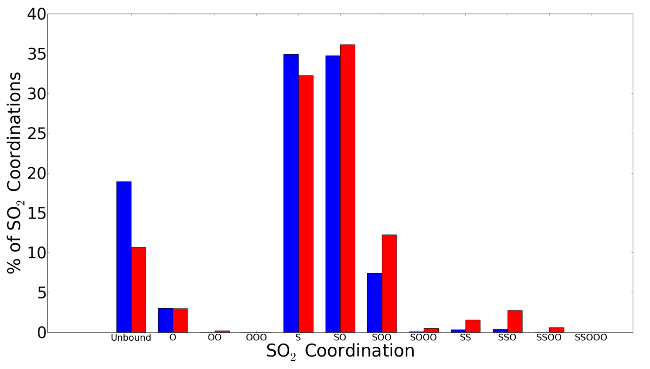
\includegraphics[scale=1.0]{images/coordinations/so2-coordinations-percents-small.png}
		\caption{The \suldiox~bonding coordinations occur with different frequencies at the surface under hot and cold temperature conditions. Shown above is the distribution of bonding coordinations of the cold (blue) and hot (red) \suldiox~over the entire set of trajectories. The values are the percentage of MD timesteps spent in the given bonding coordination.}
		\label{fig:bonding-coordinations}
	\end{center}
\end{figure}

	Several conclusions about the bonding behavior of \suldiox~to surface waters stem from this distribution of coordinations. Clearly the cold \suldiox~spends more time than the hot \suldiox, 13\% versus 3\%, respectively, completely unbound from the surface waters. This does not necessarily imply a complete desorption into the gas phase, but only a brief sojourn away from the waters, with all interactions and bond lengths longer than the cutoff criteria used for the analysis. Furthermore, the most frequently occurring bonding coordinations are ``S'',``SO'', and ``SOO'', with ``SO'' being the most populated at both temperatures. Baer et al. also concluded that these three coordinations were the most frequent for a room temperature simulation, and specifically identified the ``SO'' and ``SOO'' as most common in their study.\cite{Baer2010}

	Looking closer at the coordination types it is notable that coordinations lacking any sulfur interactions (i.e. ``O'', ``OO'', etc.) represent the least frequently formed. A bonding coordination with at least a single sulfur interaction is clearly favored over \suldiox~``oxygen-only'' bonding to waters. In our previous classical simulations of \suldiox~on water we concluded that during adsorption and throughout the interface, the \suldiox~orients so that its sulfur tends to the \wat~bulk side of the interface.\cite{Shamay2011} The coordination distributions here support the idea that binding through the sulfur is preferable, and to the extent that a non-sulfur coordination is rarely formed during the course of all our simulations.

% Baer's assymetric oxygen binding
Baer et al performed this coordination analysis for their single-temperature study, but discriminated between \suldiox~binding through the two different oxygens. They concluded that there is asymmetric hydrogen bonding through the \suldiox~oxygens, with one binding more often than the other. This is supported by the findings here where all the double oxygen coordinations (i.e. ``OO'', ``SOO'', etc.) represent a much lower percentage of the coordinations than the single oxygen counterparts (i.e. ``O'', ``SO'', etc.). Furthermore, a triple-oxygen coordination (i.e. ``OOO'', ``SOOO'', etc.) is very rarely encountered. Three \suldiox~oxygen bonds only form if both \suldiox~oxygens are interacting with water hydrogens. Our finding that triple-oxygen coordinations rarely form complements Baer et al's conclusion about the asymmetry in the oxygen interactions.

Having established the preference for an interaction through the \suldiox~sulfur atom, we look to the right side of Figure \ref{fig:bonding-coordinations} at the double-sulfur coordinations (i.e. ``SS'', ``SSO'', ``SSOO'', etc.). We see from the data that single-sulfur coordinations are overwhelmingly preferred over double-sulfur ones. Adding a third oxygen atom is also unfavorable as the ``OOO'' and ``SSOOO'' represent less than 1\% of the trajectories, and the comparison between ``SOO'' to ``SOOO'' shows a very large decrease in occurrences.

We can now form a picture of a typical \suldiox~molecule adsorbed to a water surface across both temperatures in this study. The \suldiox~will have at least one interaction to neighboring waters through the sulfur, and will then bond asymmetrically through one of the oxygens either once or twice to water hydrogens. The \suldiox~oxygen bonds will form and break repeatedly throughout a trajectory, and overall the most dominant coordination will be the ``SO'' bonding arrangement.


\subsection {Temperature Effects on Bonding Coordinations}

The binding behavior of the \suldiox~is altered by changing the temperature of the system, as evidenced in the shift in bonding coordination populations of Figure \ref{fig:bonding-coordinations} from cold to hot. In the cold temperature, the unbound, ``S'', and ``SO'' coordinations are more populated than in the hot systems. The increased temperature decreases the time spent in the unbound coordination, and causes all the coordinations to the right of ``SO'' in Figure \ref{fig:bonding-coordinations} to increase over the equivalent cold temperature populations. We see that the cold \suldiox~spends nearly four times as much time unbound as the hot \suldiox, with most of the unbound population in the hot simulations shifting to coordinations with double-oxygen and double-sulfur bonds. 

On the cold water surface, the ``S'' and ``SO'' are more populated than for the hot system. The relative decrease of these coordinations are matched in the hot surface by an increase of the ``SOO'' configuration. This speaks to a dramatic difference in the surface behavior of \suldiox~at the two temperatures. The cold \suldiox~spends nearly equal time in the ``S'' and ``SOO'' coordinations, but nearly 20\% more time in the ``SO''. Thus, the addition or removal of a bond through the \suldiox-oxygen to a neighboring coordination (i.e. addition of an oxygen bond from ``SO'' to ``SOO'', or removal of the bond from ``SO'' to ``S'') is equally probable, as long as the sulfur interaction with the water oxygen does not break. 

Figure \ref{fig:rdf} shows the radial distribution functions (RDF) of \suldiox~to water atoms for both cold (blue) and hot (red) temperatures. The S-O$_{H_2O}$ RDFs are nearly equal except for a slightly taller first peak in the cold system. Along with the slightly larger population of the cold ``S'' and ``SO'' coordinations in the cold surface, the RDF would indicate that since bonding occurs frequently through the sulfur, the cold \suldiox-sulfur interacts more closely with the surface waters. In the hot systems, the bonding coordinations with two oxygen bonds (i.e. ``SOO'', etc.) occur more frequently than in the cold system. This additional bonding through a second oxygen interaction may slightly shift neighboring hydrating waters away from the \suldiox~sulfur towards the oxygen end of the molecule. This suggests that the cold \suldiox~bonds to water's surface closer through its sulfur atom (as shown in the S-O$_{H_2O}$ RDF) and favors the more ``sulfur-centric'' bonding coordinations (i.e. ``S'', ``SO''). The increased temperature of the hot system allows the \suldiox~to bond more extensively through its oxygens to the ``SOO'' coordination. The greater interactions through the oxygens, and higher bonding coordination, may pull the \suldiox~further into the water interface and then allow for increased bonding through the sulfur, up to double-sulfur coordinations (i.e. ``SS'', ``SSO'', etc.).

\begin{figure}[h!]
	\begin{center}
		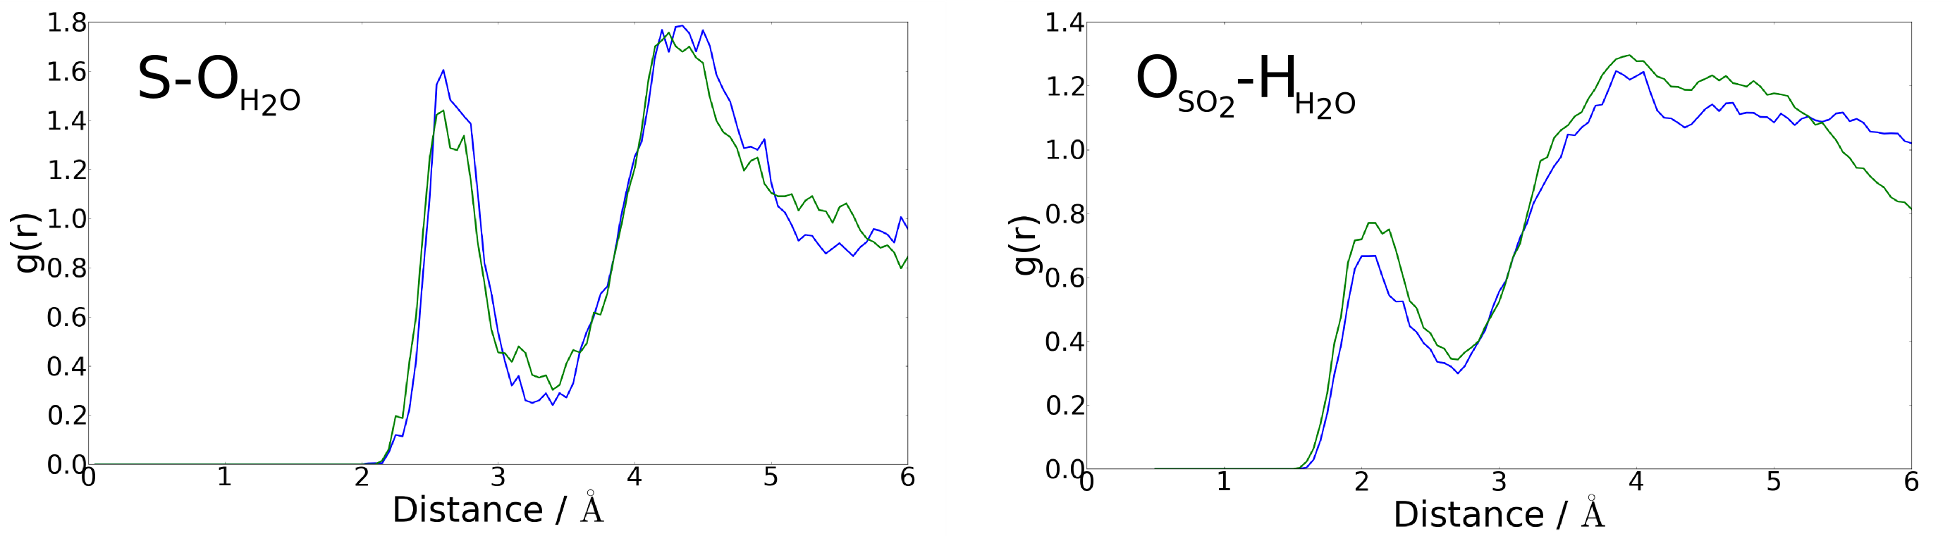
\includegraphics[scale=1.0]{images/rdf/rdf-small.png}
		\caption{Radial distribution functions (RDF) show the subtle change in how the hydrating waters around \suldiox~reposition as the temperature is increased from cold (blue) to hot (green). Shown are the two correlations between sulfur and water oxygens (left) and the \suldiox-oxygen and water hydrogens (right).}
		\label{fig:rdf}
	\end{center}
\end{figure}

\subsection {Bonding Transitions}

During the course of each cold and hot simulation, the \suldiox~bonding coordination was determined and recorded for each timestep. From the coordination data we extract not only the populations of the various bonding coordinations, but also the frequencies of transitions between the different coordinations (i.e. the number of times each \suldiox~switched from one coordination type to another). With this data we have generated the directed graphs of Figure \ref{fig:coordination-transitions} depicting the cold and hot (Figure \ref{fig:coordination-transitions} A and B, respectively) bonding coordinations as circular colored nodes.\cite{Ellson2004,Gansner1999} The transitions between the coordinations are depicted as directed edges pointing in the direction of the transition from one coordination to another. The populations of the coordinations are depicted by both the node size and coloration (larger and darker red coordinations occur more frequently). Populations of the transitions between coordinations are depicted by arrow thickness, with thicker lines corresponding to more frequently occurring transitions. Additionally, the transition lines are numbered to the right of each line with the number of times each transition occurred. 

\begin{figure}[h!]
	\begin{center}
		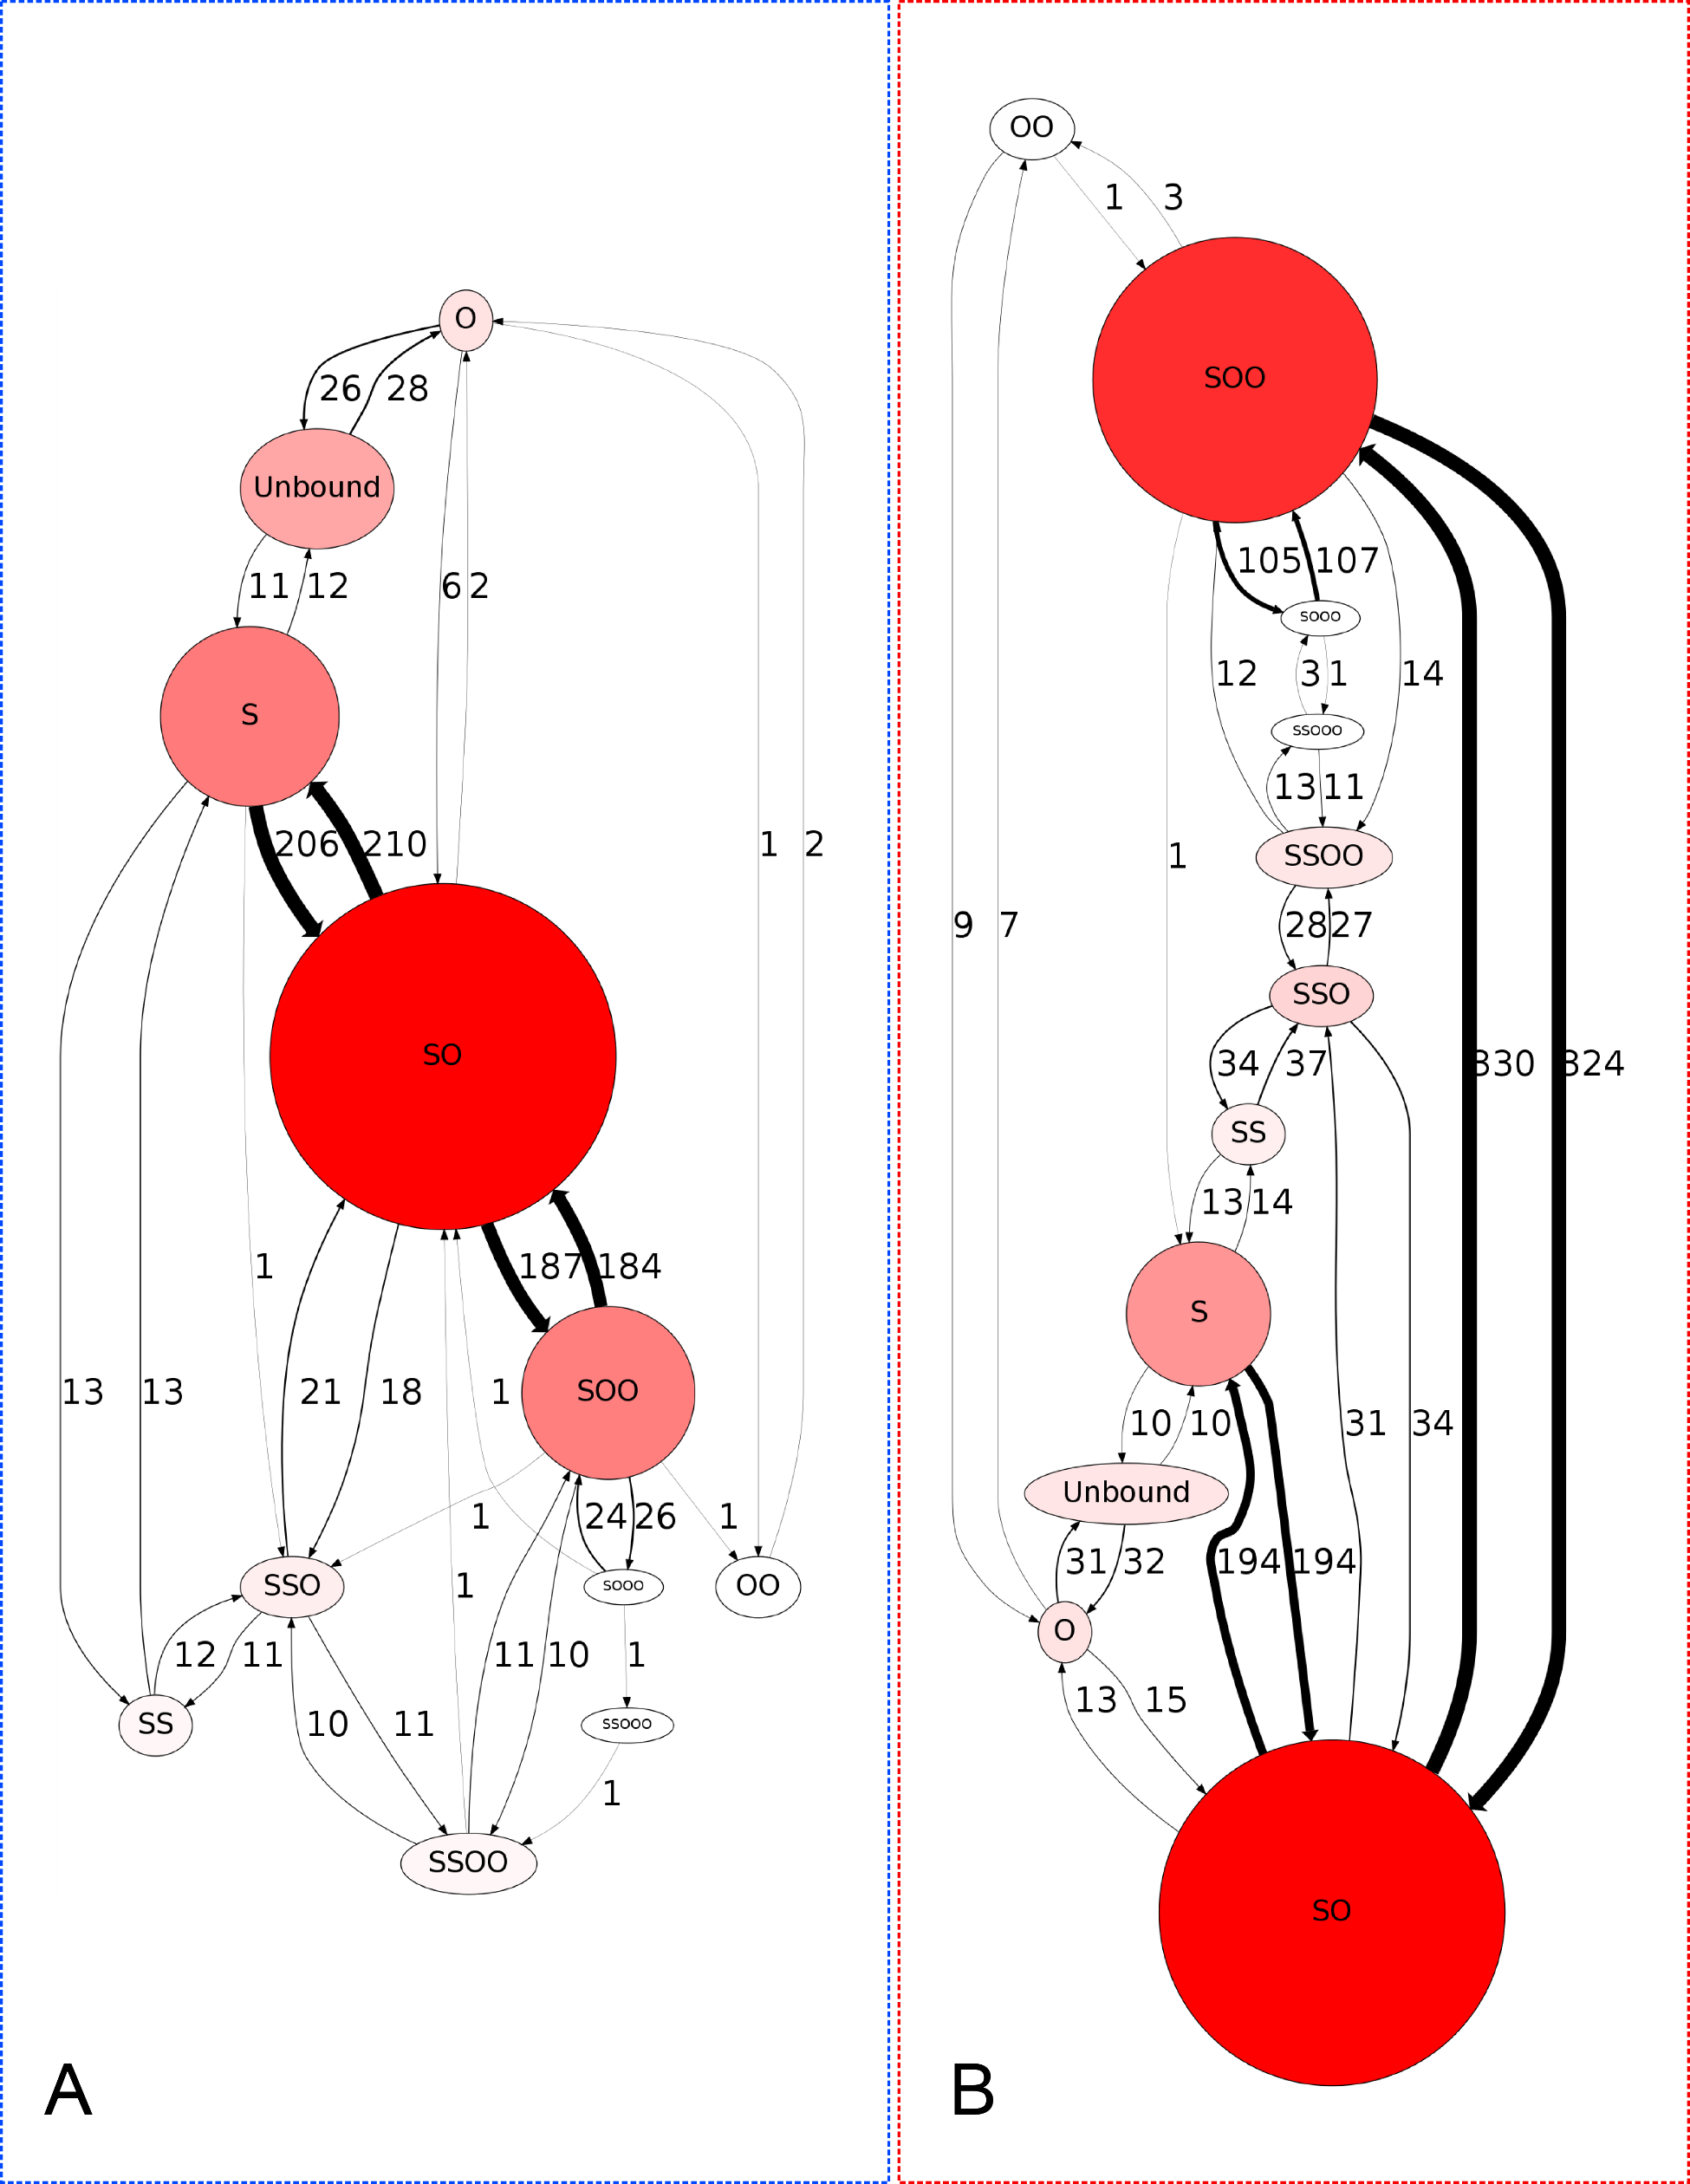
\includegraphics[scale=1.0]{images/coordinations/coordination-transitions.png}
		\caption{The bonding coordinations of \suldiox~on a water surface rapidly change as bonds break and form throughout the MD trajectories. Depicted here is a graph of the bonding coordinations, shown as colored nodes of varying size. Larger and more darkly colored coordination nodes are those more often encountered during MD (see Figure \ref{fig:bonding-coordinations}). The directed edges between the nodes represent the number of times the coordination transition occurred. Thicker lines correspond to a greater number of transitions between coordinations. The number of time a given transition occurred is labeled to the right of the corresponding line.}
		\label{fig:coordination-transitions}
	\end{center}
\end{figure}

As expected for the more populated coordinations, there are more transitions between larger nodes in Figure \ref{fig:coordination-transitions} than transitions to less populated coordinations. However, some insights to the bonding process are made clearer from these graphs. In the cold system graph of Figure \ref{fig:coordination-transitions}A, we find that the majority of transitions are between the ``S-SO'' and ``SO-SOO'' nodes. The number of transitions within this ``S-SO-SOO'' group of coordinations is an order of magnitude larger than any other transition. This indicates that while the \suldiox~is bound in any of the three most populated bonding coordinations, it is actively binding and unbinding the oxygens to form the other two coordinations in this group. Clearly, the \suldiox~is rather active and constantly forming and breaking bonds with its oxygens.

In the graph of the hot system in Figure \ref{fig:coordination-transitions}B, the transition frequencies follow the same trend as in the cold system, increasing with adjacent node size. One very surprising result is in the transition from ``SOO-SOOO''. The transition frequency does not follow from the adjacent node sizes, as the ``SOOO'' node represents less than 5\% of the bonding coordinations. This is indicative of a very rapid cycle of forming and breaking of bonds to the second \suldiox~oxygen. As noted earlier, it is likely that ``SOO'' coordinated \suldiox, asymmetrically binding twice through a single oxygen, is being pulled further into the water interface. It is likely more surrounded by waters, and in the hot system it can more easily form a brief third hydrogen bond to a water through the second \suldiox~oxygen. Because the triple-oxygen coordination is not as favorable, it quickly breaks the bond and the \suldiox~returns back to the ``SOO'' coordination.

Given the information we have about the frequencies of bonding coordination transitions, it is possible to draw a likely route of adsorption beginning with an unbound \suldiox. From the unbound coordination, the \suldiox~can bind to waters either through the sulfur or an oxygen to enter the ``S'' or ``O'' coordinations, respectively. At both temperatures we find that the coordination transition in Figure \ref{fig:coordination-transitions} from unbound to ``O'' occurs almost three times more than the transition from unbound to ``S''. We find two possibilities that may explain this difference. The ``O'' coordination may form more easily, but also break quickly after formation, accounting for the higher transition frequency. Otherwise, the ``O'' coordination may be the first step in adsorption of an unbound \suldiox, where a subsequent addition of an \suldiox~sulfur interaction to a water oxygen would lead to a transition to the most frequent coordination, ``SO''. In the latter case, any adsorption of \suldiox~may proceed through an oxygen binding, accounting for the increased unbound-``O'' transition frequency.

To verify if the ``O'' coordination forms from, and breaks quickly to the unbound coordination as is suggested by the transition frequency plots in Figure \ref{fig:coordination-transitions}, we plot the lifespans of the various coordinations in Figure \ref{fig:coordination-lifespans}. Each point in the plot represents a time during the simulation in which the \suldiox~formed the respective coordination. The vertical ``lifespan'' position is calculated directly from the amount of time spent in the given coordination before changing to another. Both cold (blue) and hot (red) simulation data are plotted. The data of Figure \ref{fig:coordination-lifespans} show that most coordination configurations last a very brief time, with the majority forming for under 0.5 ps. The three most populous coordinations, ``S'', ``SO'', ``SOO'' (as determined from Figure \ref{fig:bonding-coordinations} by percentage) in both temperatures have coordination lifetimes of up to 1 ps, in some instances lasting up to 1.5 ps. The brevity of lifespans overall speaks to the dynamic nature of the interface. The length of time in each coordination parallels the populations of the coordinations, and suggests an ordering of steady states among various bonding coordinations. The ``unbound'' configuration stands out as an anomaly amongst the lifespans of the other bonding coordinations. The few lifespans above 1.5 ps, up to 3.25 ps long, suggest a \suldiox~that not only unbinds from the water surface, but that also recedes far enough to avoid a quick rebinding and coordination change to ``S'' or ``O''. Those few long lived unbound data points indicate times when the \suldiox~is far from the water, residing in the gas phase until the necessary water rearrangement occurs and it is drawn back to the surface to rebind.

\begin{figure}[h!]
	\begin{center}
		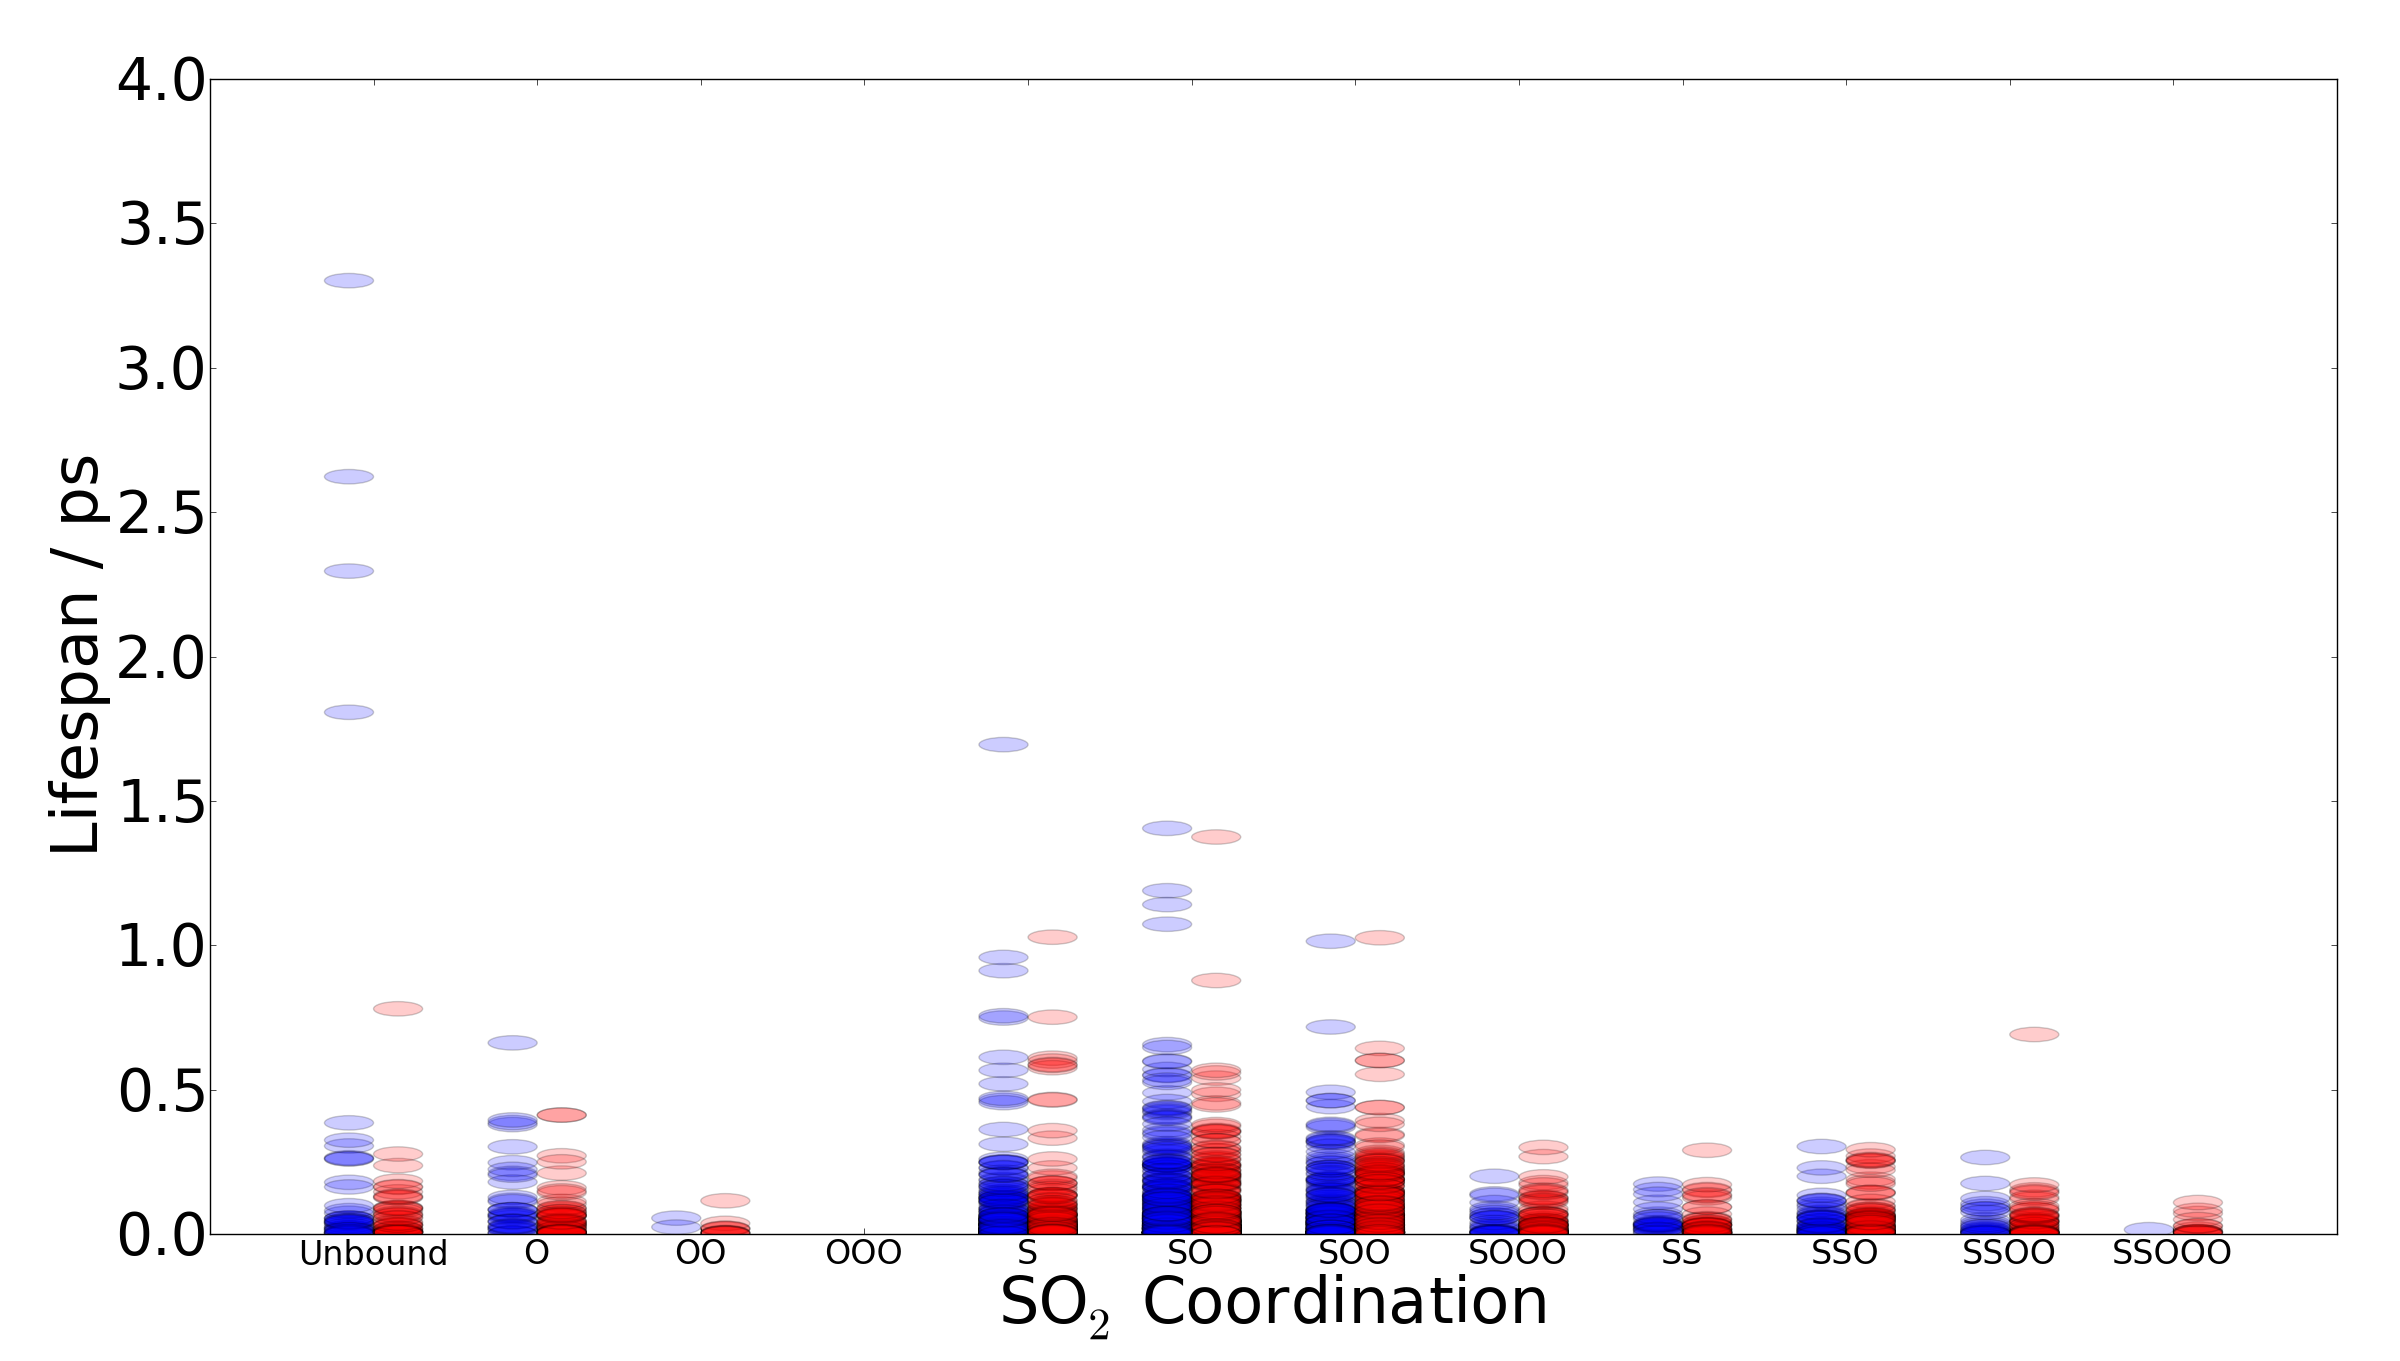
\includegraphics[scale=1.0]{images/coordinations/coordination-lifespans.png}
		\caption{Given that certain bonding coordinations of the surface \suldiox~are more often encountered than others (see Figure \ref{fig:bonding-coordinations}), the plot here shows the time spent in each bonding coordination. Each point in the plot represents a single span of simulation time that the \suldiox~had the given coordination. The amount of time spent corresponds to the vertical position along the lifespan axis, in ps.}
		\label{fig:coordination-lifespans}
	\end{center}
\end{figure}

Returning to the transition plots of Figure \ref{fig:coordination-transitions}, the behavior of the unbound transition to both ``S'' and ``O'' coordination can now be better characterized. Figure \ref{fig:coordination-lifespans} shows that the ``O'' coordinated lifetimes are shorter than the ``S'' coordinated ones. Figure \ref{fig:coordination-transitions} shows that the unbound-``O'' transition occurs almost three times more than the transition to the ``S''. The unbound \suldiox~forms a bond to a neighboring water through its oxygen, but that bond is short-lived and either quickly breaks (resulting in unbound \suldiox), or it transitions to the ``SO'' coordination by forming another bond through the sulfur. The unbound-``S'' transition does not occur as often. This may be because the ``S'' coordination is more stable than the ``O''. Once in the ``S'' coordination the \suldiox~does not quickly break the interaction from its sulfur to water, but rather remains for up to 1 ps in the ``S'' coordination before (most likely) forming an oxygen bond to make the ``SO'' coordination. We have outlined the likely behavior of \suldiox~as it transitions from the gas phase in an unbound coordination to binding to an aqueous interface by forming bonds and interactions with surface waters.

Once the \suldiox~begins interacting with the water surface, the pathway leading back to the unbound coordination is not often traversed. As shown in Figure \ref{fig:coordination-transitions} the dominant coordination transitions occur between the ``S-SO-SOO'' group of coordinations. This suggests that the \suldiox~sulfur interaction to a water oxygen has a much longer lifespan than the oxygen bonding to water hydrogens. The difference between the ``S-SO-SOO'' coordinations is an addition or removal of oxygen bonds, and the frequent transitions between them show that the bonds to \suldiox~oxygens are quickly forming and breaking. For the \suldiox~sulfur interaction to break, the \suldiox~must enter a non-sulfur coordination (i.e. ``O'', ``OO'', unbound, etc.) or a coordination with more than a single sulfur interaction (i.e. ``SS'', ``SSO'', etc.). The transitions to coordinations that allow for breaking of the \suldiox~sulfur interactions, or switching the interaction to another water, are infrequent compared to those leading to an oxygen bond transition. Thus, the \suldiox~spends most of its time while bound to the surface waters breaking and forming hydrogen-bonds through its oxygens, and interacting with neighboring waters through a more persistent interaction via the \suldiox~sulfur atom.
